\begin{frame}
  \maketitle
\end{frame}

\begin{frame}
  \frametitle{Piano della presentazione}
  \tableofcontents
\end{frame}

\section{Introduzione}

\begin{frame}
  \frametitle{Cos'è?}
  \begin{block}{Energia oscura}
    Forma di energia che permea l'Universo.
  \end{block}
  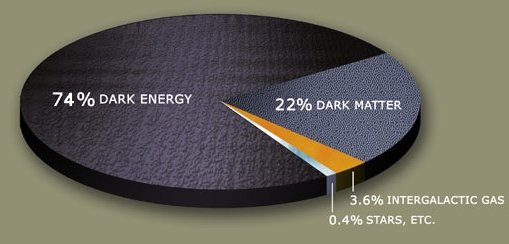
\includegraphics[width=\columnwidth]{DarkMatterPie}
\end{frame}

\section[Origine]{Origine dell'energia oscura}

\begin{frame}
  \frametitle{Perché serve l'energia oscura?}
  L'Universo si sta espandendo in maniera \alert{accelerata}.
  \begin{figure}
    \centering
    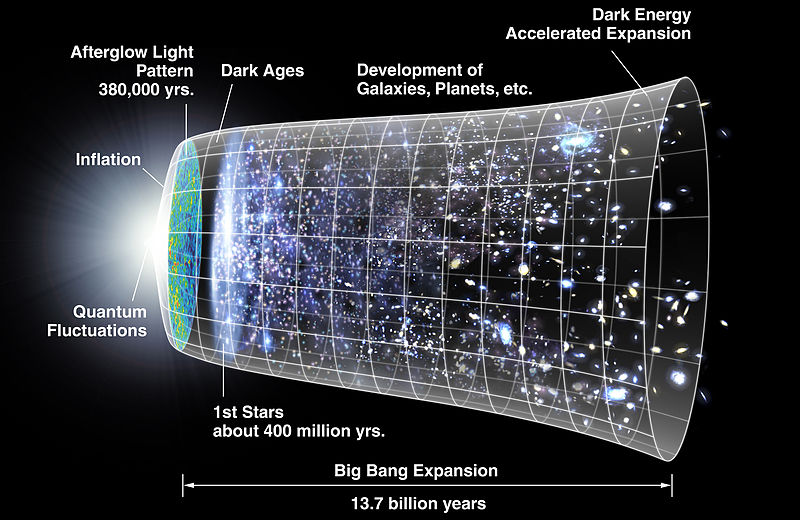
\includegraphics[width=0.9\columnwidth]{800px-CMB_Timeline300_no_WMAP}
  \end{figure}
\end{frame}

\begin{frame}
  \frametitle{Prove dell'espansione accelerata dell'Universo}
  \begin{itemize}
  \item Supernove di tipo Ia (Riess 1998 e Perlmutter 1999)
  \item Radiazione cosmica di fondo
  \item Struttura a grande scala dell'Universo
  \item Microlensing gravitazionale
  \end{itemize}
\end{frame}

\section[Natura]{Natura dell'energia oscura}

\begin{frame}
  \frametitle{Cos'è precisamente l'energia oscura?}
  Ci sono varie ipotesi
  \begin{itemize}
  \item Costante cosmologica
  \item Quintessenza
  \item Altre idee alternative
  \end{itemize}
\end{frame}

\begin{frame}
  \frametitle{Che caratteristiche ha?}
  Indipendentemente dalle ipotesi sulla natura l'energia oscura deve avere
  \alert{pressione negativa}. Serve per giustificare l'accelerazione
  nell'espansione.
\end{frame}

\begin{frame}
  \frametitle[]{Equazioni fondamentali}
  Particella di massa $m$, mezzo in espansione di massa $M = 4\pi\rho r^3/3$.
  \begin{align*}
    F &= \frac{GMm}{r^2} = \frac{4\pi G \rho r m}{3} \\
    V &= -\frac{GMm}{r} = -\frac{4\pi G \rho r^2 m}{3} \\
    T &= \frac{1}{2}m\dot{r} \\
    U &= T + V = \frac{1}{2}m\dot{r} - \frac{4\pi G \rho r^2 m}{3}
  \end{align*}
  Poniamo $\vec{r} = R(t)\vec{x}$ e $kc^2 = -2U/mx^2$.
\end{frame}

\begin{frame}
  \frametitle{Equazioni fondamentali}
  \begin{block}{Equazione di Friedmann}
    \begin{equation*}
      H^2 = \left( \frac{\dot{R}}{R} \right)^2 = \frac{8\pi G}{3}\rho -
      \frac{kc^2}{a^2}
    \end{equation*}
  \end{block}
  \pause{}
  \begin{block}{Equazione del fluido (conservazione energia)}
    \begin{equation*}
      \dot{\rho} + 3\frac{\dot{R}}{R}\left( \rho + \frac{p}{c^2} \right) = 0
    \end{equation*}
  \end{block}
  \pause{}
  \begin{block}{Equazione di accelerazione}
    \begin{equation*}
    \frac{\ddot{R}}{R} = -\frac{4\pi G}{3}\left( \rho + \frac{3p}{c^2} \right)
  \end{equation*}
  \end{block}
  Non tutte indipendenti.
\end{frame}

\begin{frame}
  \frametitle{Curvatura}
  \begin{table}
    \centering
    \begin{tabular}{ccc}
      \toprule{}
      Curvatura & Geometria & Universo \\
      \midrule{}
      $k < 0$ & sferica & chiuso \\
      $k = 0$ & piana & piatto \\
      $k > 0$ & iperbolica & aperto \\
      \bottomrule{}
    \end{tabular}
  \end{table}
\end{frame}

\begin{frame}
  \frametitle{Costante cosmologica}
  L'equazione di Friedmann da sola \\
  non spiega l'accelerazione nell'espansione.
  \begin{block}{Equazione di Friedmann modificata}
    \begin{equation*}
      H^2 = \frac{8\pi G}{3}\rho - \frac{kc^2}{R^2} + \frac{\Lambda}{3}
    \end{equation*}
  \end{block}
  Costante cosmologica già introdotta da Einstein per provare a spiegare un
  Universo statico.
\end{frame}

\begin{frame}
  \frametitle{Fluido cosmologico}
  Universo è riempito da un fluido di densità
  \begin{equation*}
    \rho(t) = \rho_{\textup{m}}(t) + \rho_{\textup{r}}(t) + \rho_\Lambda(t)
  \end{equation*}
  \pause{}
  \begin{block}{Componenti del fluido}
    \begin{equation*}
      \rho_{\textup{m}}(t) =
      \underbrace{\rho_{\textup{stelle}}(t) +
        \rho_{\textup{nucleosintesi}}(t)}_{\rho_{\textup{barioni}(t)}} +
      \rho_{\textup{materia oscura}}(t)
    \end{equation*}
    \pause{}
    \begin{equation*}
      \rho_{\textup{r}}(t) = \rho_\gamma(t) + \rho_\nu(t)
    \end{equation*}
    \pause{}
    \begin{equation*}
      \rho_\Lambda = \frac{\Lambda c^2}{8\pi G}
    \end{equation*}
  \end{block}
\end{frame}

\begin{frame}
  \frametitle{Fluido cosmologico}
  Per ciascuna componente del fluido si può scrivere
  \begin{block}{Equazione di stato}
    \begin{equation*}
      p_i = w_i \rho_i c^2
    \end{equation*}
  \end{block}
  \pause{}
  Inserendo nell'equazione dei fluidi
  \begin{block}{Evoluzione dei fluidi}
    \begin{equation*}
      \rho \propto \frac{1}{R^{3(1+w)}}
    \end{equation*}
  \end{block}
  \pause{}
  Materia: $w = 0 \implies \rho \propto 1/R^3$ \\
  \pause{}
  Radiazione: $w = 1/3 \implies \rho \propto 1/R^4$ \\
  \pause{}
  Energia oscura (vuoto): $w = -1 \implies \rho \text{ costante}$
\end{frame}

\begin{frame}
  \frametitle{Parametro di densità}
  \begin{block}{Parametro di densità}
    \begin{equation*}
      \Omega_i(t) = \frac{\rho_i(t)}{\rho_{\textup{crit}}} = \frac{8\pi
        G}{3H^2(t)}\rho_i(t)
    \end{equation*}
  \end{block}
  \pause{}
  Sperimentalmente si è trovato
  \begin{equation*}
    \Omega_{\textup{m},0} \approx \num{0.3} \qquad \Omega_{\textup{r},0} \approx
    \num{5e-5} \qquad \Omega_\Lambda \approx \num{0.7}
  \end{equation*}
  L'energia oscura domina l'Universo!
\end{frame}

% TODO: grafico (con Tikz è meglio)q 7.1, pag 54 del Liddle. Mostrare dove ci
% troviamo noi oggi (\Omega = 1 !)

\begin{frame}
  \frametitle{Quintessenza}
  La costante cosmologica ha \\
  densità costante in spazio e tempo. \\
  Se invece ammettiamo che possa variare \\
  abbiamo $p_{\textup{Q}} = w\rho_{\textup{Q}}c^2$ \\
  con $w \neq 1$ e $w < -1/3$ affinché \\
  la pressione negativa permetta l'espansione accelerata. \\
  In questo caso l'energia oscura si chiama \alert{quintessenza}.
\end{frame}

\section[Conseguenze]{Conseguenze nel destino dell'Universo}

\begin{frame}
  \frametitle{Quale sarà la fine dell'Universo?}
  Dipende fortemente dalla reale densità di energia e materia oscure.
  \begin{figure}
    \centering
    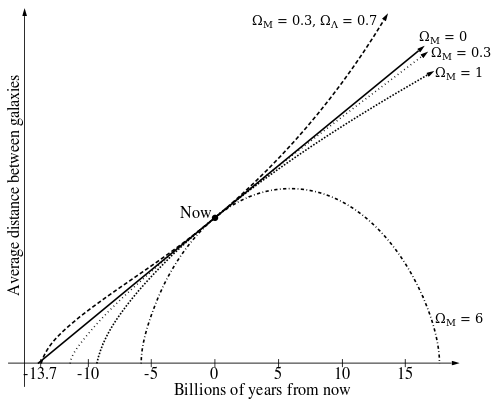
\includegraphics[width=0.7\columnwidth]{500px-Friedmann_universes}
  \end{figure}
\end{frame}

\section{Problemi aperti}

\begin{frame}
  \frametitle{Cosa c'è ancora da scoprire?}
  \begin{itemize}[<+->]
  \item Qual è il valore $k$ della curvatura?
  \item L'espansione sta realmente accelerando?
  \item L'energia oscura è l'energia quantistica del vuoto?
  \end{itemize}
\end{frame}

%%% Local Variables:
%%% mode: latex
%%% TeX-master: "seminario"
%%% End:
